\documentclass{report}

\usepackage{amsmath}
\usepackage{amssymb}

\usepackage{tikz}
\usetikzlibrary{intersections, calc,through,backgrounds}

\usepackage{titlesec}
\usepackage[skins]{tcolorbox}
\usepackage{xcolor}

% colors
%%%%%%%%%%%%%%%%%%%%%%%%%%%%%%%%%%%%%%%%%%%%%%%%%%%%%%%%%%
\definecolor{i}{HTML}{FF0000}
\definecolor{j}{HTML}{00BB00}
\definecolor{k}{HTML}{0000FF}

\definecolor{1}{HTML}{1F77B4}
\definecolor{2}{HTML}{FF7F0E}
\definecolor{3}{HTML}{2CA02C}

\definecolor{problem}{HTML}{FFFCAB}
\definecolor{problem_frame}{HTML}{BBCC00}
%%%%%%%%%%%%%%%%%%%%%%%%%%%%%%%%%%%%%%%%%%%%%%%%%%%%%%%%%%

\newcommand{\bi}{\vec{i}}
\newcommand{\bj}{\vec{j}}
\newcommand{\bk}{\vec{k}}

%--------------------------------------------------

%define a new environment for problem statements
\newsavebox{\selvestebox}
\newenvironment{colbox}[1]
  {\newcommand\colboxcolor{#1}%
   \begin{lrbox}{\selvestebox}%
   \begin{minipage}{\dimexpr\columnwidth-2\fboxsep\relax}}
  {\end{minipage}\end{lrbox}%
   \begin{center}
   \fcolorbox{problem!50!black}{\colboxcolor}{\usebox{\selvestebox}}
   \end{center}}
   
\newcommand{\problem}[1]{\begin{colbox}{problem}#1\end{colbox}}

\title{\textsc{Problem Set 1}\\Vectors and Matrices}
\begin{document}

\maketitle



\subsection*{1A-10}
\problem{Prove using vector methods (without components) that the 
midpoints of the sides of a space quadrilateral form a parallelogram.}

Lets take the points $O$, $P$, $Q$, and $R$ as the verticies of a 
quadrilateral, as illustrated below. 

\begin{figure}[!h]
\centering
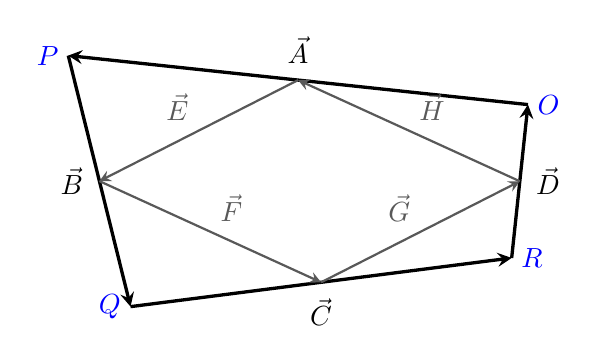
\begin{tikzpicture}
    [Vector qd/.style={->, very thick, color=black},
     Vector pg/.style={->, thick, color=black!65},
    >=stealth
    ]
%declare points OPQR at random locations
\coordinate[label=right:\textcolor{blue}{$O$}] (O) at ($(0,0) + (rand, rand)$);
\coordinate[label=left:\textcolor{blue}{$P$}] (P) at ($(-5,0) + (rand, rand)$);
\coordinate[label=left:\textcolor{blue}{$Q$}] (Q) at ($(-5,-3) + (rand, rand)$);
\coordinate[label=right:\textcolor{blue}{$R$}] (R) at ($(0,-3) + (rand, rand)$);

\coordinate (S) at ($(O)!0.5!(P)$);
\coordinate (T) at ($(P)!0.5!(Q)$);
\coordinate (U) at ($(Q)!0.5!(R)$);
\coordinate (V) at ($(R)!0.5!(O)$);

\draw[Vector qd, name=A]  (O) -- node[above=2pt]{$\vec{A}$} (P);
\draw[Vector qd, name=B]  (P) -- node[left=2pt]{$\vec{B}$} (Q);
\draw[Vector qd, name=C]  (Q) -- node[below=2pt]{$\vec{C}$} (R);
\draw[Vector qd, name=D]  (R) -- node[right=2pt]{$\vec{D}$} (O);

\draw[Vector pg]  (S) -- node[above left]{$\vec{E}$} (T);
\draw[Vector pg]  (T) -- node[above right]{$\vec{F}$} (U);
\draw[Vector pg]  (U) -- node[above left]{$\vec{G}$} (V);
\draw[Vector pg]  (V) -- node[above right]{$\vec{H}$} (S);

\end{tikzpicture}
\end{figure}

Consider the vectors that run along the edges, pointing in the counterclockwise
direction, labelled $\vec{A}$, $\vec{B}$, $\vec{C}$, and $\vec{D}$. 
In particular, 
\begin{align*}
\vec{A} = \vec{OP} = P - O\hspace{5em}
\vec{B} = \vec{PQ} = Q - P\\ 
\vec{C} = \vec{QR} = R - Q\hspace{5em}
\vec{D} = \vec{RO} = O - R
\end{align*}

Let $\vec{E}$ be vector connecting the midpoints of $OP$ and $PQ$.
Which, in terms of $\vec{A}$ and $\vec{B}$, becomes 
\[\vec{E} = \frac{1}{2}(\vec{A} + \vec{B})\]
Similarly, the vector connecting the midpoints of $QR$ and $RO$, which
we will denote $\vec{G}$, can be expressed as 
\[\vec{G} = \frac{1}{2}(\vec{C} + \vec{D})\]

Now if we expand out $\vec{A} + \vec{B}$, we get
\begin{align*} 
\vec{A} + \vec{B} &= \vec{OP} + \vec{PQ}\\
                  &= P - O + Q - P\\
                  &=  Q - O \\
                  &=  \vec{OQ} \\
\end{align*}

Meanwhile, expanding $\vec{C} + \vec{D}$ yeilds
\begin{align*} 
\vec{C} + \vec{D} &= \vec{QR} + \vec{RO}\\ 
                  &= R - Q + O - R\\ 
                  &=  O - Q \\
                  &=  \vec{QO} \\
                  &=  -\vec{OQ} \\
\end{align*} 

Thus $\vec{A} + \vec{B} = -(\vec{C} + \vec{D})$.
Which is to say the vectors $\vec{E}$ and $\vec{G}$ run anti-parrallel 
and have the same magnitude. By the same process we can deduce 
$\vec{B}+\vec{C} = -(\vec{D}+\vec{A})$. 
Which in turn means that the vectors $\vec{H}$ and $\vec{F}$ also run 
anti-parallel  and have the same magnitude.

Therefore we the shape formed by connecting the midpoints of a 
quadrilateral is a parallelogram.


\end{document}
